\documentclass[10.5pt,a4paper]{article}
\usepackage[utf8]{inputenc}
\usepackage[T1]{fontenc}
\IfFileExists{brazil.ldf}{\usepackage[brazil]{babel}}{}
\usepackage{charter}
\renewcommand{\ttdefault}{pcr}
\usepackage[a4paper,top=2cm,bottom=2cm,left=2.2cm,right=2.2cm]{geometry}
\usepackage{microtype}
\usepackage{amsmath,amssymb}
\usepackage{booktabs}
\usepackage{tabularx}
\usepackage{multirow}
\usepackage{enumitem}
\usepackage[dvipsnames,table]{xcolor}
\usepackage{titlesec}
\usepackage{fancyhdr}
\usepackage{listings}
\usepackage[most]{tcolorbox}
\usepackage{tikz}
\usetikzlibrary{positioning,arrows.meta,calc}
\usepackage{pgfplots}
\pgfplotsset{compat=1.17}
\usepgfplotslibrary{groupplots}
\usepackage{xstring}
\usepackage{catchfile}
\usepackage[font=small,labelfont=bf,labelsep=colon]{caption}
\captionsetup[figure]{name=Figura}
\captionsetup[table]{name=Tabela}
\usepackage{xurl}
\usepackage[colorlinks=true,linkcolor=azul,urlcolor=azul,citecolor=azul]{hyperref}

% =====================================================================
% numeros_finais.tex
% Gerado pelo pipeline (scripts/gerar_numeros_latex.py) apos o corte.
% NAO editar a mao: rodar o script e recompilar o PDF.
% =====================================================================
\newcommand{\statusprevisao}{FINAL (corte 03/10/2026 20h00)}
\newcommand{\npesquisas}{6}
\newcommand{\listapesquisas}{Datafolha (BR-00304/2026 e BR-08039/2026), Quaest (BR-06520/2026), PoderData (BR-01739/2026), AtlasIntel (BR-04391/2026) e Real Time Big Data (BR-09503/2026)}

% Modelo oficial (votos validos, %)
\newcommand{\pLula}{45,6}
\newcommand{\pFlavio}{45,9}
\newcommand{\pCury}{2,6}
\newcommand{\pCaiado}{2,6}
\newcommand{\pRenan}{2,5}
\newcommand{\pZema}{0,7}
\newcommand{\pSamara}{0,1}
\newcommand{\pClariana}{0,0}
\newcommand{\pEdmilson}{0,0}
\newcommand{\pHertz}{0,0}
\newcommand{\pRui}{0,0}
\newcommand{\pWilson}{0,0}

% M0 puro (sensibilidade)
\newcommand{\mLula}{45,4}
\newcommand{\mFlavio}{41,5}
\newcommand{\mCury}{4,1}
\newcommand{\mCaiado}{3,0}
\newcommand{\mRenan}{3,9}
\newcommand{\mZema}{1,1}

% Aba 2
\newcommand{\pAbst}{22,3}
\newcommand{\pBrancos}{1,6}
\newcommand{\pNulos}{2,8}


% Sensibilidade (definidos pelo pipeline em numeros_finais.tex; valores abaixo so entram se o pipeline nao os definir)
\providecommand{\sViesLula}{44,5}\providecommand{\sViesFlavio}{44,8}
\providecommand{\sUtilLula}{46,5}\providecommand{\sUtilFlavio}{42,5}
\providecommand{\sNanLula}{45,5}\providecommand{\sNanFlavio}{45,8}

\definecolor{azul}{HTML}{1F3A5F}
\definecolor{azulclaro}{HTML}{E8EEF5}
\definecolor{cinza}{HTML}{555555}
\definecolor{cinzaclaro}{HTML}{B5B5B5}
\definecolor{vermelho}{HTML}{B03A2E}
\definecolor{verde}{HTML}{2E7D4F}
\definecolor{codebg}{HTML}{F6F8FA}

\titleformat{\section}{\normalfont\Large\bfseries\color{azul}}{\thesection}{0.6em}{}
\titleformat{\subsection}{\normalfont\large\bfseries\color{azul!85!black}}{\thesubsection}{0.5em}{}
\titlespacing*{\section}{0pt}{14pt}{6pt}
\titlespacing*{\subsection}{0pt}{10pt}{4pt}
\setlength{\parindent}{0pt}
\setlength{\parskip}{5pt}
\setlist{itemsep=2pt,topsep=3pt,leftmargin=1.4em}

\pagestyle{fancy}
\fancyhf{}
\renewcommand{\headrulewidth}{0pt}
\fancyhead[R]{\footnotesize\color{cinza}Relatório técnico: previsão do 1º turno de 2026}
\fancyfoot[L]{\footnotesize\color{cinza}Valuche, Possamai e Lyra}
\fancyfoot[R]{\footnotesize\color{cinza}\thepage}

\lstdefinestyle{py}{
  language=Python, basicstyle=\ttfamily\footnotesize, backgroundcolor=\color{codebg},
  keywordstyle=\color{azul}\bfseries, commentstyle=\color{cinza}, stringstyle=\color{verde},
  showstringspaces=false, frame=single, rulecolor=\color{black!12}, framesep=4pt,
  xleftmargin=6pt, xrightmargin=6pt, breaklines=true, columns=fullflexible, keepspaces=true,
  literate={á}{{\'a}}1 {é}{{\'e}}1 {í}{{\'i}}1 {ó}{{\'o}}1 {ú}{{\'u}}1 {ã}{{\~a}}1 {õ}{{\~o}}1 {ç}{{\c{c}}}1 {Í}{{\'I}}1
}
\lstset{style=py}

\newtcolorbox{destaque}[1][]{colback=azulclaro,colframe=azul,boxrule=0.6pt,arc=2pt,left=6pt,right=6pt,top=4pt,bottom=4pt,#1}

% numeros com ponto para graficos
\newcommand{\dif}[2]{\StrSubstitute{#1}{,}{.}[\difA]\StrSubstitute{#2}{,}{.}[\difB]\pgfmathsetmacro{\difR}{\difA-\difB}\pgfmathprintnumber[fixed,precision=1,fixed zerofill,use comma,showpos]{\difR}}
\newcommand{\pontodec}[2]{\StrSubstitute{#1}{,}{.}[#2]}
\pontodec{\pLula}{\dLula}\pontodec{\pFlavio}{\dFlavio}\pontodec{\pCury}{\dCury}\pontodec{\pCaiado}{\dCaiado}
\pontodec{\pRenan}{\dRenan}\pontodec{\pZema}{\dZema}\pontodec{\pSamara}{\dSamara}\pontodec{\pClariana}{\dClariana}
\pontodec{\pEdmilson}{\dEdmilson}\pontodec{\pHertz}{\dHertz}\pontodec{\pRui}{\dRui}\pontodec{\pWilson}{\dWilson}
\pontodec{\mLula}{\eLula}\pontodec{\mFlavio}{\eFlavio}\pontodec{\mCury}{\eCury}\pontodec{\mCaiado}{\eCaiado}
\pontodec{\mRenan}{\eRenan}\pontodec{\mZema}{\eZema}

\begin{document}

%================= CAPA =================
\begin{tcolorbox}[colback=azul,colframe=azul,arc=0pt,left=14pt,right=14pt,top=14pt,bottom=14pt]
\color{white}
{\small DESAFIO DE ESTATÍSTICA E ECONOMETRIA \textbullet\ FGV EPGE}\\[6pt]
{\huge\bfseries Previsão do 1º turno presidencial de 2026}\\[4pt]
{\Large Relatório técnico completo}\\[10pt]
{\normalsize João Pedro Valuche de Andrade Pereira \textbullet\ Lethicia Manfioletti Possamai \textbullet\ Arthur Caron Lyra}
\end{tcolorbox}

\vspace{4pt}
\begin{destaque}
\textbf{Horário de corte dos dados: sábado, 03/10/2026, às 20h00 (horário de Brasília).} Status: \statusprevisao.

Este relatório detalha o que a nota metodológica de duas páginas resume: os dados, cada etapa do código, todos os modelos testados, os resultados completos da validação e as limitações. Todos os números vêm do mesmo código que gera a planilha de entrega.
\end{destaque}

\vspace{4pt}
{\setlength{\tabcolsep}{0pt}
\begin{tabularx}{\linewidth}{@{}*{6}{>{\centering\arraybackslash}X}@{}}
\textcolor{azul}{\huge\bfseries \pFlavio\%} & \textcolor{azul}{\huge\bfseries \pLula\%} & \textcolor{azul}{\huge\bfseries \pCury\%} & \textcolor{cinza}{\huge\bfseries \pAbst\%} & \textcolor{cinza}{\huge\bfseries \pBrancos\%} & \textcolor{cinza}{\huge\bfseries \pNulos\%}\\[2pt]
\small Flávio Bolsonaro & \small Lula & \small Augusto Cury & \small Abstenção & \small Brancos & \small Nulos
\end{tabularx}}

\vspace{6pt}
\setcounter{tocdepth}{1}
{\small\tableofcontents}

\newpage
%================= 1 =================
\section{O problema}

Precisamos prever, para o 1º turno de 4 de outubro de 2026, o percentual de votos válidos de cada um dos $K=12$ candidatos e três agregados: a abstenção (sobre o eleitorado apto) e os votos brancos e nulos (sobre o comparecimento). O erro de uma previsão é o erro absoluto médio sobre todos os candidatos:
\begin{equation}
\text{MAE}=\frac{1}{K}\sum_{i=1}^{K}\left|\hat p_i-p_i\right|.
\label{eq:mae}
\end{equation}

Duas consequências guiaram o trabalho. Primeiro, o vencedor importa pouco: errar Lula e Flávio em 2 pontos cada pesa o mesmo que errar quatro candidatos médios em 1 ponto cada. Segundo, os candidatos pequenos contam: com 12 candidatos, um erro de 0,5 ponto em cada um dos sete nanicos soma 3,5 pontos, mais do que um erro grande em um dos líderes. Por isso escolhemos modelos pelo MAE sobre \emph{toda} a urna das eleições passadas, incluindo os candidatos que as pesquisas nem divulgavam.

%================= 2 =================
\section{Dados}

\subsection{Resultados oficiais}
Baixamos do Portal de Dados Abertos do TSE a votação por candidato e o detalhe da apuração de 2006, 2010, 2014, 2018 e 2022 e agregamos ao nível nacional. Como teste de sanidade, o código reproduz os números oficiais de 2022 (Lula 48,43\%, Bolsonaro 43,20\%, abstenção 20,95\%) e falha se algum deles divergir.

\subsection{Pesquisas históricas}
Reunimos 109 pesquisas nacionais estimuladas de 1º turno divulgadas nos 21 dias anteriores a cada eleição, com instituto, datas de campo e divulgação, amostra e contratante. Duas decisões de limpeza:
\begin{itemize}
\item o \emph{tracking} diário do Vox Populi em 2010 foi reduzido a rodadas sem sobreposição de amostra, para não contar o mesmo entrevistado várias vezes;
\item Ibope e Ipec formam uma única série, já que o Ipec foi criado pela equipe do Ibope.
\end{itemize}

\subsection{Pesquisas de 2026}
Usamos somente pesquisas com registro conferido no PesqEle/TSE. Cada número foi transcrito da página original, que guardamos com hash SHA-256; um teste automático confere cada valor transcrito junto ao nome do candidato na página salva. A Tabela~\ref{tab:pesq26} lista as pesquisas, em votos totais, como foram divulgadas.

\IfFileExists{tabela_pesquisas_2026.tex}{\CatchFileDef{\tabpesq}{tabela_pesquisas_2026.tex}{}%
\begin{table}[h]
\centering\small
\caption{Pesquisas de 2026 usadas (\% dos votos totais, como divulgadas). Na média entra a mais recente de cada instituto.}
\label{tab:pesq26}
\footnotesize\setlength{\tabcolsep}{3pt}
\begin{tabular}{llcrcccccccc}
\toprule
Instituto & Registro TSE & Campo & $n$ & Lula & Flávio & Cury & Caiado & Renan & Zema & B+N & Indec. \\
\midrule
\tabpesq
\bottomrule
\end{tabular}
\end{table}}{}

%================= 3 =================
\section{Pipeline}

A Figura~\ref{fig:pipe} mostra o caminho dos dados até a planilha. Cada caixa é uma função testada no repositório; a seguir mostramos versões resumidas do código, sem docstrings e tratamento de casos extremos.

\begin{figure}[h]
\centering
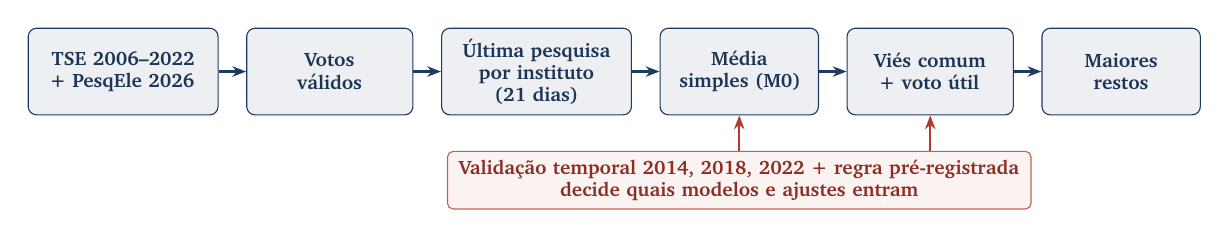
\begin{tikzpicture}[node distance=0.35cm,
  caixa/.style={rectangle,rounded corners=3pt,draw=azul,fill=azul!8,text=azul!90!black,align=center,font=\scriptsize\bfseries,inner sep=3pt,minimum height=1.1cm},
  seta/.style={-{Stealth[length=5pt]},thick,azul},
  faixa/.style={rectangle,rounded corners=2pt,draw=vermelho!80,fill=vermelho!6,text=vermelho!80!black,align=center,font=\scriptsize\bfseries,inner sep=3pt}]
\node[caixa,text width=2.2cm] (a) {TSE 2006--2022\\+ PesqEle 2026};
\node[caixa,text width=1.9cm,right=of a] (b) {Votos\\válidos};
\node[caixa,text width=2.2cm,right=of b] (c) {Última pesquisa\\por instituto\\(21 dias)};
\node[caixa,text width=1.8cm,right=of c] (d) {Média\\simples (M0)};
\node[caixa,text width=1.9cm,right=of d] (e) {Viés comum\\+ voto útil};
\node[caixa,text width=1.8cm,right=of e] (f) {Maiores\\restos};
\foreach \x/\y in {a/b,b/c,c/d,d/e,e/f} \draw[seta] (\x)--(\y);
\node[faixa,below=0.45cm of d,text width=7.2cm] (v) {Validação temporal 2014, 2018, 2022 + regra pré-registrada\\decide quais modelos e ajustes entram};
\draw[seta,vermelho] (v.north -| d) -- (d);
\draw[seta,vermelho] (v.north -| e) -- (e);
\end{tikzpicture}
\caption{Do dado bruto à previsão. Em vermelho, a etapa que decide o que entra no modelo.}
\label{fig:pipe}
\end{figure}

\subsection{Conversão para votos válidos}
Cada pesquisa divulga intenções $x_{ij}$ em votos totais, incluindo brancos, nulos e indecisos. Convertemos para votos válidos dividindo pela soma dos candidatos:
\begin{equation}
v_{ij}=\frac{x_{ij}}{\sum_{c=1}^{K}x_{cj}}\times 100 .
\end{equation}
Isso equivale a supor que os indecisos se distribuem como os decididos, a mesma hipótese implícita na apuração do TSE.
\begin{lstlisting}
def converter_para_votos_validos(linha, candidatos):
    intencoes = {c: float(linha.get(c)) if pd.notna(linha.get(c)) else 0.0
                 for c in candidatos}
    soma = sum(intencoes.values())          # brancos, nulos e indecisos ficam fora
    if soma <= 0:
        raise ValueError("Soma das intenções é zero")
    return {c: v / soma * 100.0 for c, v in intencoes.items()}
\end{lstlisting}

\subsection{Agregação (M0)}
De cada instituto usamos só a pesquisa mais recente dentro da janela, para que institutos com rodadas frequentes não pesem mais que os outros. A previsão base é a média simples entre institutos.
\begin{lstlisting}
def estimar_m0(df_pesquisas, eleicao):
    df = df_pesquisas.copy()
    df["instituto_clean"] = df["instituto"].apply(padronizar_nome_instituto)
    ultimas = (df.sort_values("data_divulgacao", ascending=False)
                 .drop_duplicates(subset=["instituto_clean"]))   # 1 por instituto
    validos = [converter_pesquisa_validos(r, candidatos) for _, r in ultimas.iterrows()]
    media = {c: np.mean([p[c] for p in validos]) for c in candidatos}
    return renormalizar_votos(media)
\end{lstlisting}

\subsection{Arredondamento}
A planilha exige uma casa decimal e soma exata de 100,0. Arredondar cada valor separadamente pode dar 99,9 ou 100,1. Usamos o método dos maiores restos: arredondamos todos para baixo e distribuímos os décimos que faltam aos candidatos com as maiores partes descartadas.
\begin{lstlisting}
def maiores_restos(valores, total=100.0, casas=1):
    fator = 10 ** casas
    escalados = [round(v * total / sum(valores) * fator, 10) for v in valores]
    inteiros  = [math.floor(s) for s in escalados]
    faltam    = round(total * fator) - sum(inteiros)
    ordem = sorted(range(len(valores)), key=lambda i: (-(escalados[i] - inteiros[i]), i))
    for i in ordem[:faltam]:
        inteiros[i] += 1                     # décimo vai para o maior resto
    return [x / fator for x in inteiros]
\end{lstlisting}

%================= 4 =================
\section{Modelos candidatos}

Antes de rodar qualquer validação, registramos por escrito quatro modelos base e suas grades de hiperparâmetros.

\paragraph{M0, média simples.} $\hat p_i=\frac{1}{J}\sum_{j=1}^{J}v_{ij}$, com $J$ institutos.

\paragraph{M1, recência e amostra.} Pesquisas maiores e mais próximas da eleição pesam mais:
\begin{equation}
\hat p_i=\frac{\sum_j w_j v_{ij}}{\sum_j w_j},\qquad w_j=\sqrt{N_j}\;2^{-\Delta t_j/h},\qquad h\in\{7,14,21\}\text{ dias},
\end{equation}
em que $N_j$ é a amostra e $\Delta t_j$ a distância em dias até a véspera. A raiz de $N_j$ vem de o erro amostral cair com $1/\sqrt{N}$.

\paragraph{M2, efeito instituto (\emph{house effect}).} Alguns institutos erram sistematicamente para um lado. Para cada instituto $j$ e bloco político $b\in\{\text{PT},\text{principal adversário},\text{demais}\}$, medimos o desvio médio do instituto em relação à média dos institutos na mesma eleição, $\bar\beta_{jb}$, e o encolhemos conforme o número de eleições $n_j$ em que o instituto aparece:
\begin{equation}
\hat\beta_{jb}=\frac{n_j}{n_j+k}\,\bar\beta_{jb},\qquad k\in\{1,3,10\},\qquad v^{\text{corr}}_{ij}=v_{ij}-\hat\beta_{j,b(i)} .
\end{equation}
Medir o desvio contra a média dos institutos, e não contra a urna, separa o efeito do instituto do erro que todos cometem juntos (tratado na Seção~\ref{sec:final}).

\paragraph{M3, regressão Ridge.} Regressão do resultado de cada candidato sobre a média das pesquisas, a incumbência (candidato ou partido do governo) e a posição nas pesquisas, com penalização $\alpha\|\beta\|_2^2$, $\alpha\in\{0{,}1;\,1;\,10\}$.

%================= 5 =================
\section{Protocolo de validação}

\subsection{Validação temporal}
Uma previsão eleitoral só pode usar o passado. Por isso validamos em janela crescente (\emph{expanding window}): cada eleição de teste é prevista usando só as anteriores (Figura~\ref{fig:ew}). Como complemento, reportamos também o \emph{leave-one-election-out} (LOEO), que usa as cinco eleições mas deixa cada uma de fora por vez.

\begin{figure}[h]
\centering
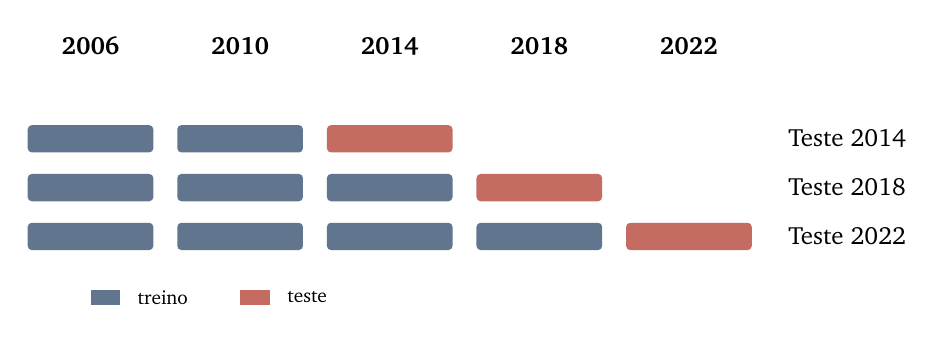
\begin{tikzpicture}[x=1.9cm,y=0.62cm]
\foreach \a [count=\i] in {2006,2010,2014,2018,2022} \node[font=\small\bfseries] at (\i,0.9) {\a};
\foreach \r/\t/\lab in {1/3/{Teste 2014},2/4/{Teste 2018},3/5/{Teste 2022}}{
  \pgfmathtruncatemacro{\last}{\t-1}
  \foreach \c in {1,...,\last} \fill[azul!70,rounded corners=1.5pt] (\c-0.42,-\r+0.28) rectangle (\c+0.42,-\r-0.28);
  \fill[vermelho!75,rounded corners=1.5pt] (\t-0.42,-\r+0.28) rectangle (\t+0.42,-\r-0.28);
  \node[anchor=west,font=\small] at (5.6,-\r) {\lab};
}
\fill[azul!70] (1,-4.1) rectangle (1.2,-4.4); \node[anchor=west,font=\scriptsize] at (1.25,-4.25) {treino};
\fill[vermelho!75] (2,-4.1) rectangle (2.2,-4.4); \node[anchor=west,font=\scriptsize] at (2.25,-4.25) {teste};
\end{tikzpicture}
\caption{Janela crescente: nenhuma previsão usa informação posterior à eleição prevista. São 21, 39 e 69 pesquisas de treino e 18, 30 e 40 pesquisas de teste.}
\label{fig:ew}
\end{figure}

\subsection{Regra de decisão}
Com só três eleições de teste, uma diferença pequena de MAE pode ser ruído. Fixamos a regra antes de ver os resultados. Para comparar um modelo mais complexo $B$ com um mais simples $A$, calculamos a redução do erro em cada eleição, $\Delta_t=\text{MAE}^A_t-\text{MAE}^B_t$, e exigimos
\begin{equation}
\bar\Delta>\text{EP}(\Delta)=\frac{s_\Delta}{\sqrt{n}},\qquad n=3 .
\label{eq:regra}
\end{equation}
Se a condição não vale, fica o mais simples, na ordem M0, M1, M2, M3. A decisão é sequencial: primeiro escolhemos o modelo base; depois testamos cada ajuste sobre ele, um de cada vez; por fim, o modelo combinado.
\begin{lstlisting}
def calcular_diferenca_e_se(mae_A, mae_B):
    deltas = np.array(mae_A) - np.array(mae_B)     # ganho de B sobre A, por eleição
    s_delta = np.std(deltas, ddof=1)
    return deltas.mean(), s_delta / math.sqrt(len(deltas))
\end{lstlisting}

\subsection{Pré-registro}
O documento de pré-registro, com os modelos, as grades e a regra acima, foi escrito antes do backtest e recebeu três emendas datadas, todas anteriores à execução da validação: a primeira tratou das datas de divulgação, dos nanicos divulgados de forma agregada, da separação entre instituto e contratante e do teste de sanidade das vésperas; a segunda escreveu as equações, as grades e a regra de empate, e definiu o viés comum, o voto útil e a âncora dos nanicos; a terceira separou o efeito instituto do viés comum, fixou o protocolo sequencial e a tabela de incumbência. Depois de rodar o backtest, nenhum modelo ou hiperparâmetro foi alterado.

%================= 6 =================
\section{Resultados da validação}

\subsection{Etapa 1: modelo base}
A Tabela~\ref{tab:etapa1} traz todas as configurações. A média simples teve o menor erro em 2014 e 2018 e o menor erro médio. O segundo colocado, M1 com $h=7$, perde por $\bar\Delta=0{,}27$ ponto com $\text{EP}=0{,}21$: escolhemos o M0.

\begin{table}[h]
\centering\small
\caption{Etapa 1: MAE (p.p.) no \emph{expanding window}, todas as configurações.}
\label{tab:etapa1}
\begin{tabular}{llcccc}
\toprule
Modelo & Configuração & 2014 & 2018 & 2022 & Média \\
\midrule
\rowcolor{azulclaro} M0 & média simples & 1,33 & 1,50 & 0,83 & \textbf{1,22} \\
M1 & $h=7$ & 1,96 & 1,73 & 0,77 & 1,49 \\
   & $h=14$ & 2,08 & 1,85 & 0,81 & 1,58 \\
   & $h=21$ & 2,13 & 1,89 & 0,83 & 1,62 \\
M2 & $k=1$ & 2,09 & 1,82 & 0,92 & 1,61 \\
   & $k=3$ & 2,09 & 1,83 & 0,85 & 1,59 \\
   & $k=10$ & 2,09 & 1,84 & 0,82 & 1,58 \\
M3 & $\alpha=0{,}1$ & 2,01 & 1,89 & 1,36 & 1,75 \\
   & $\alpha=1$ & 1,85 & 2,02 & 1,19 & 1,69 \\
   & $\alpha=10$ & 1,99 & 2,13 & 1,26 & 1,79 \\
\bottomrule
\end{tabular}
\end{table}

\begin{figure}[h]
\centering
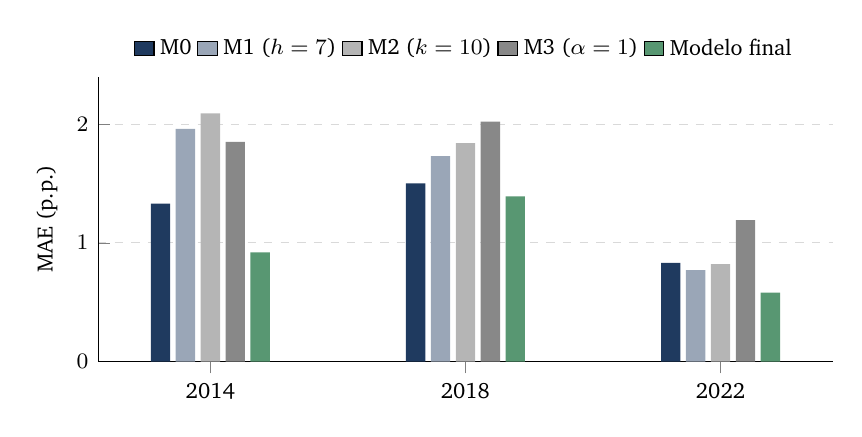
\begin{tikzpicture}
\begin{axis}[width=0.9\linewidth,height=5.2cm,ybar,bar width=7pt,
  symbolic x coords={2014,2018,2022},xtick=data,ymin=0,ymax=2.4,
  ylabel={MAE (p.p.)},enlarge x limits=0.22,ymajorgrids,grid style={dashed,gray!30},axis lines*=left,
  legend style={draw=none,font=\footnotesize,at={(0.5,1.02)},anchor=south,legend columns=5},
  /pgf/number format/use comma,tick label style={font=\footnotesize},label style={font=\footnotesize},
  legend image code/.code={\draw[#1] (0cm,-0.08cm) rectangle (0.25cm,0.1cm);}]
\addplot[fill=azul,draw=none] coordinates {(2014,1.33) (2018,1.50) (2022,0.83)};
\addplot[fill=azul!45,draw=none] coordinates {(2014,1.96) (2018,1.73) (2022,0.77)};
\addplot[fill=cinzaclaro,draw=none] coordinates {(2014,2.09) (2018,1.84) (2022,0.82)};
\addplot[fill=cinza!70,draw=none] coordinates {(2014,1.85) (2018,2.02) (2022,1.19)};
\addplot[fill=verde!80,draw=none] coordinates {(2014,0.92) (2018,1.39) (2022,0.58)};
\legend{M0,M1 ($h=7$),M2 ($k=10$),M3 ($\alpha=1$),Modelo final}
\end{axis}
\end{tikzpicture}
\caption{MAE por eleição da melhor configuração de cada modelo e do modelo final. Os modelos mais sofisticados erram mais que a média simples em 2014 e 2018: com poucas eleições para estimar pesos e efeitos, a complexidade extra vira ruído.}
\label{fig:mae}
\end{figure}

\subsection{Etapa 2: ajustes sobre o M0}
\begin{table}[h]
\centering\small
\caption{Etapa 2: cada ajuste testado isoladamente sobre o M0 e o modelo combinado.}
\label{tab:etapa2}
\begin{tabular}{lccccccl}
\toprule
Configuração & 2014 & 2018 & 2022 & Média & $\bar\Delta$ & EP & Decisão \\
\midrule
M0 (referência) & 1,33 & 1,50 & 0,83 & 1,22 & & & \\
\midrule
Viés comum, $k_\mu=1$ & 1,08 & 1,43 & 0,88 & 1,13 & 0,09 & 0,09 & passa \\
\rowcolor{azulclaro} Viés comum, $k_\mu=3$ & 0,95 & 1,45 & 0,71 & 1,04 & 0,18 & 0,10 & passa (melhor) \\
Viés comum, $k_\mu=10$ & 1,13 & 1,48 & 0,69 & 1,10 & 0,12 & 0,05 & passa \\
\midrule
Voto útil, $\gamma=0{,}25$ & 1,33 & 1,48 & 0,76 & 1,19 & 0,03 & 0,02 & passa \\
Voto útil, $\gamma=0{,}5$ & 1,32 & 1,46 & 0,68 & 1,16 & 0,07 & 0,04 & passa \\
\rowcolor{azulclaro} Voto útil, $\gamma=1$ & 1,31 & 1,43 & 0,53 & 1,09 & 0,13 & 0,09 & passa (melhor) \\
\midrule
Âncora dos nanicos, $w=0{,}5$ & 1,31 & 1,50 & 0,84 & 1,22 & 0,004 & 0,007 & não passa \\
\midrule
\rowcolor{verde!12} \textbf{Modelo final} & \textbf{0,92} & \textbf{1,39} & \textbf{0,58} & \textbf{0,96} & \textbf{0,26} & \textbf{0,09} & \textbf{adotado} \\
\bottomrule
\end{tabular}
\end{table}

A âncora dos nanicos (mediana histórica dos partidos equivalentes no TSE) não passou na regra: as pesquisas antigas quase nunca divulgavam nanicos individualmente, então não havia como medir o ganho. Fixamos $w=0$.

O LOEO confirma o resultado: o modelo final tem MAE médio de 1,24 contra 1,45 do M0 e erra menos em quatro das cinco eleições (2006, 2014, 2018 e 2022).

\subsection{Erro candidato a candidato}
A Figura~\ref{fig:cand} mostra onde o modelo final ganha e onde perde. Em 2014 ele reduz bastante o erro de Dilma e de Aécio. Em 2018 corrige quase todo o erro de Bolsonaro, mas piora o de Haddad. Em 2022 passa do ponto em Bolsonaro e piora Lula, mas reduz o erro de Tebet e Ciro, e o saldo no MAE ainda é positivo.

\begin{figure}[h]
\centering
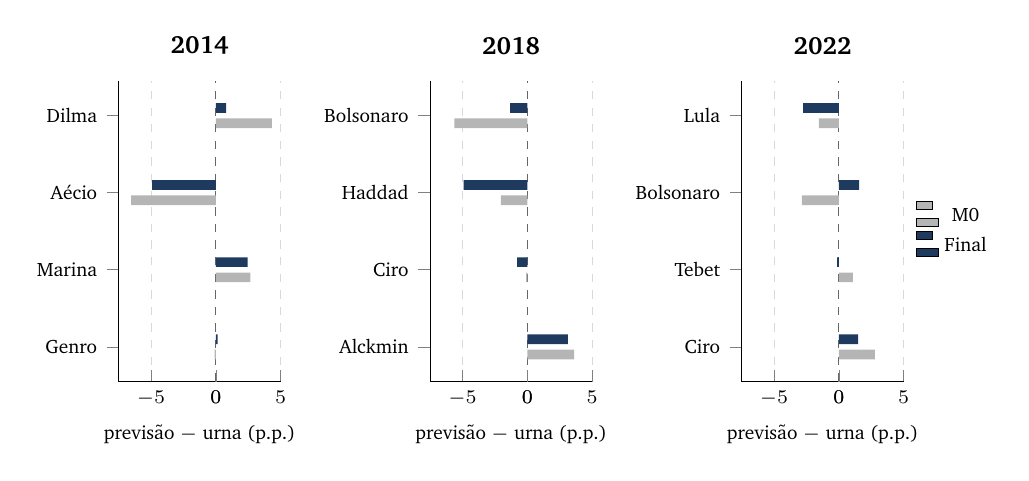
\begin{tikzpicture}
\begin{groupplot}[group style={group size=3 by 1,horizontal sep=1.9cm},
  width=0.30\linewidth,height=5.4cm,xbar,/pgf/bar width=3.5pt,xmin=-7.5,xmax=5,
  ytick=data,tick label style={font=\scriptsize},title style={font=\small\bfseries},
  xmajorgrids,grid style={dashed,gray!30},axis lines*=left,enlarge y limits=0.15,
  extra x ticks={0},extra x tick style={grid=major,major grid style={black!60}},
  xlabel={previsão $-$ urna (p.p.)},label style={font=\scriptsize}]
\nextgroupplot[title=2014,symbolic y coords={Genro,Marina,Aécio,Dilma}]
\addplot[fill=cinzaclaro,draw=none] coordinates {(-0.10,Genro) (2.66,Marina) (-6.55,Aécio) (4.33,Dilma)};
\addplot[fill=azul,draw=none] coordinates {(0.14,Genro) (2.46,Marina) (-4.92,Aécio) (0.80,Dilma)};
\nextgroupplot[title=2018,symbolic y coords={Alckmin,Ciro,Haddad,Bolsonaro}]
\addplot[fill=cinzaclaro,draw=none] coordinates {(3.61,Alckmin) (-0.09,Ciro) (-2.05,Haddad) (-5.63,Bolsonaro)};
\addplot[fill=azul,draw=none] coordinates {(3.12,Alckmin) (-0.79,Ciro) (-4.92,Haddad) (-1.34,Bolsonaro)};
\nextgroupplot[title=2022,symbolic y coords={Ciro,Tebet,Bolsonaro,Lula},legend style={draw=none,font=\scriptsize,at={(1.02,0.5)},anchor=west}]
\addplot[fill=cinzaclaro,draw=none] coordinates {(2.79,Ciro) (1.08,Tebet) (-2.85,Bolsonaro) (-1.55,Lula)};
\addplot[fill=azul,draw=none] coordinates {(1.48,Ciro) (-0.13,Tebet) (1.57,Bolsonaro) (-2.76,Lula)};
\legend{M0,Final}
\end{groupplot}
\end{tikzpicture}
\caption{Erro dos quatro candidatos mais votados em cada eleição de teste, média simples (cinza) e modelo final (azul).}
\label{fig:cand}
\end{figure}

%================= 7 =================
\section{O modelo final}
\label{sec:final}

\subsection{Viés comum}
As pesquisas de véspera não erram ao acaso: nas três eleições de teste, o principal adversário do PT terminou acima da média das pesquisas (Figura~\ref{fig:vies}). Como todos os institutos erraram para o mesmo lado, o efeito instituto do M2 não captura esse erro; é um erro da eleição inteira. Estimamos o viés médio de cada bloco nas eleições de treino e o subtraímos da média de 2026:
\begin{equation}
\hat\mu_b=\frac{N}{N+k_\mu}\cdot\frac{1}{N}\sum_{t=1}^{N}\left(\bar v^{\,\text{pesq}}_{b,t}-v^{\,\text{TSE}}_{b,t}\right),\qquad k_\mu=3,\qquad \hat p_i\leftarrow \hat p_i-\hat\mu_{b(i)} .
\end{equation}
O fator $N/(N+3)$ encolhe a correção quando há poucas eleições de treino: com $N=2$, aplicamos 40\% do viés médio; com $N=5$, 62,5\%.

\begin{lstlisting}
def aplicar_ajuste_vies_comum(base_preds, eleicao, eleicoes_treino, k_mu=3.0):
    erros = {"pt": [], "adv": [], "demais": []}
    for t in eleicoes_treino:                       # só eleições anteriores
        tse = carregar_resultado_tse(t)
        for _, row in obter_pesquisas_eleicao(t).iterrows():
            p = converter_pesquisa_validos(row, HISTORICO_CANDIDATOS[t])
            for c in HISTORICO_CANDIDATOS[t]:
                erros[identificar_bloco(t, c)].append(p[c] - tse[c])
    n = len(eleicoes_treino)
    mu = {b: n / (n + k_mu) * np.mean(e) for b, e in erros.items()}
    ajustado = {c: max(0.0, v - mu[identificar_bloco(eleicao, c)])
                for c, v in base_preds.items()}
    return renormalizar_votos(ajustado)
\end{lstlisting}

\begin{figure}[h]
\centering
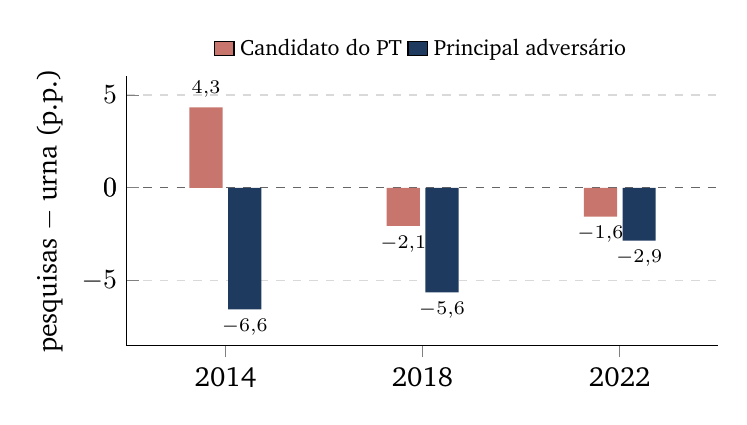
\begin{tikzpicture}
\begin{axis}[width=0.75\linewidth,height=5cm,ybar,bar width=12pt,
  symbolic x coords={2014,2018,2022},xtick=data,ymin=-8.5,ymax=6,
  ylabel={pesquisas $-$ urna (p.p.)},enlarge x limits=0.25,ymajorgrids,grid style={dashed,gray!30},axis lines*=left,
  extra y ticks={0},extra y tick style={grid=major,major grid style={black!60}},
  nodes near coords,nodes near coords style={font=\scriptsize,/pgf/number format/fixed,/pgf/number format/precision=1,/pgf/number format/fixed zerofill},
  /pgf/number format/use comma,legend style={draw=none,font=\footnotesize,at={(0.5,1.02)},anchor=south,legend columns=2},
  legend image code/.code={\draw[#1] (0cm,-0.08cm) rectangle (0.25cm,0.1cm);}]
\addplot[fill=vermelho!70,draw=none] coordinates {(2014,4.33) (2018,-2.05) (2022,-1.55)};
\addplot[fill=azul,draw=none] coordinates {(2014,-6.55) (2018,-5.63) (2022,-2.85)};
\legend{Candidato do PT,Principal adversário}
\end{axis}
\end{tikzpicture}
\caption{Erro da média simples das pesquisas de véspera. O principal adversário do PT (Aécio em 2014, Bolsonaro em 2018 e 2022) foi subestimado nas três eleições.}
\label{fig:vies}
\end{figure}

\subsection{Voto útil}
Na reta final, parte dos eleitores do 3º e do 4º colocados migra para um dos dois primeiros, que têm chance real de ir ao 2º turno. Medimos a perda média $\bar\delta$ dos candidatos em 3º e 4º entre a média das pesquisas e a urna nas eleições de treino e a transferimos aos dois primeiros, na proporção das intenções:
\begin{equation}
\hat p_{3,4}\leftarrow \hat p_{3,4}-\gamma\bar\delta\,\frac{\hat p_{3,4}}{\hat p_3+\hat p_4},\qquad
\hat p_{1,2}\leftarrow \hat p_{1,2}+\gamma\bar\delta\,\frac{\hat p_{1,2}}{\hat p_1+\hat p_2},\qquad \gamma=1 .
\end{equation}
\begin{lstlisting}
transf = gamma * delta_bar
adj[c3] -= transf * base[c3] / (base[c3] + base[c4])    # sai do 3o e 4o
adj[c4] -= transf * base[c4] / (base[c3] + base[c4])
adj[c1] += transf * base[c1] / (base[c1] + base[c2])    # entra no 1o e 2o
adj[c2] += transf * base[c2] / (base[c1] + base[c2])
\end{lstlisting}

%================= 8 =================
\section{Previsão de 2026}

\begin{figure}[h]
\centering
\begin{tikzpicture}
\begin{axis}[width=0.92\linewidth,height=8.2cm,xbar,bar width=5pt,xmin=0,xmax=54,
  symbolic y coords={Wilson Grassi,Rui Costa Pimenta,Hertz Dias,Edmilson Costa,Clariana Barão,Samara Martins,Romeu Zema,Renan Santos,Ronaldo Caiado,Augusto Cury,Lula,Flávio Bolsonaro},
  ytick={Wilson Grassi,Rui Costa Pimenta,Hertz Dias,Edmilson Costa,Clariana Barão,Samara Martins,Romeu Zema,Renan Santos,Ronaldo Caiado,Augusto Cury,Lula,Flávio Bolsonaro},tick label style={font=\footnotesize},xlabel={\% dos votos válidos},label style={font=\footnotesize},
  nodes near coords,nodes near coords style={font=\scriptsize,/pgf/number format/fixed,/pgf/number format/precision=1,/pgf/number format/fixed zerofill},
  /pgf/number format/use comma,xmajorgrids,grid style={dashed,gray!30},axis lines*=left,enlarge y limits=0.05,
  legend style={draw=none,font=\footnotesize,at={(0.97,0.3)},anchor=east},reverse legend,
  legend image code/.code={\draw[#1] (0cm,-0.08cm) rectangle (0.25cm,0.1cm);}]
\addplot[fill=cinzaclaro,draw=none] coordinates {(\eZema,Romeu Zema) (\eRenan,Renan Santos) (\eCaiado,Ronaldo Caiado) (\eCury,Augusto Cury) (\eLula,Lula) (\eFlavio,Flávio Bolsonaro)};
\addplot[fill=azul,draw=none] coordinates {(\dWilson,Wilson Grassi) (\dRui,Rui Costa Pimenta) (\dHertz,Hertz Dias) (\dEdmilson,Edmilson Costa) (\dClariana,Clariana Barão) (\dSamara,Samara Martins) (\dZema,Romeu Zema) (\dRenan,Renan Santos) (\dCaiado,Ronaldo Caiado) (\dCury,Augusto Cury) (\dLula,Lula) (\dFlavio,Flávio Bolsonaro)};
\legend{Média simples (M0),Modelo final}
\end{axis}
\end{tikzpicture}
\caption{Previsão de 2026 para os 12 candidatos.}
\label{fig:prev}
\end{figure}

\begin{table}[h]
\centering\small
\caption{Previsão final e decomposição: quanto cada ajuste desloca Lula e Flávio.}
\label{tab:sens}
\begin{tabular}{lccc}
\toprule
Configuração & Lula & Flávio & Lula $-$ Flávio (p.p.) \\
\midrule
M0 (média simples) & \mLula & \mFlavio & \dif{\mLula}{\mFlavio} \\
M0 + viés comum & \sViesLula & \sViesFlavio & \dif{\sViesLula}{\sViesFlavio} \\
M0 + voto útil & \sUtilLula & \sUtilFlavio & \dif{\sUtilLula}{\sUtilFlavio} \\
\rowcolor{azulclaro}\textbf{Modelo final} & \textbf{\pLula} & \textbf{\pFlavio} & \textbf{\dif{\pLula}{\pFlavio}} \\
Modelo final com âncora dos nanicos ($w=0{,}5$) & \sNanLula & \sNanFlavio & \dif{\sNanLula}{\sNanFlavio} \\
\bottomrule
\end{tabular}
\end{table}

A decomposição mostra que o viés comum é o ajuste que mais move a previsão: sozinho, leva Flávio para perto de Lula. O voto útil puxa votos de Cury, Caiado e Renan para os dois primeiros. A âncora dos nanicos, que ficou de fora pela regra, quase não muda o resultado.

\paragraph{Margem entre os dois primeiros.} No backtest, o erro do modelo final na margem entre 1º e 2º colocados foi de 5,72 pontos em 2014, 3,58 em 2018 e 4,32 em 2022 (média de 4,5). A diferença prevista entre Lula e Flávio é bem menor que isso: o modelo não tem resolução para apontar quem termina em primeiro.

\paragraph{Faixas de erro.} No backtest, o erro absoluto ficou abaixo de 4,9 pontos em 80\% dos casos para os dois primeiros colocados, de 2,5 pontos para o 3º e o 4º e de 0,6 ponto para os demais.

%================= 9 =================
\section{Abstenção, brancos e nulos}

Para cada agregado comparamos três previsores na mesma janela crescente e com a mesma regra: persistência ($\hat y_t=y_{t-1}$), média histórica ($\hat y_t=\frac{1}{|T|}\sum_{s\in T}y_s$) e tendência linear (regressão em função do ano). A ordem de simplicidade é persistência, média, tendência.

\begin{table}[h]
\centering\small
\caption{Erro absoluto (p.p.) por eleição de teste e decisão.}
\begin{tabular}{llccccl}
\toprule
Variável & Método & 2014 & 2018 & 2022 & Média & Decisão \\
\midrule
\multirow{3}{*}{Abstenção} & Persistência & 1,27 & 0,94 & 0,62 & 0,94 & \\
 & Média & 1,96 & 2,24 & 2,30 & 2,17 & \\
 & \cellcolor{azulclaro}Tendência & \cellcolor{azulclaro}0,10 & \cellcolor{azulclaro}0,40 & \cellcolor{azulclaro}0,70 & \cellcolor{azulclaro}\textbf{0,40} & vence: $\bar\Delta=0{,}54>\text{EP}=0{,}36$ \\
\midrule
\multirow{3}{*}{Brancos} & \cellcolor{azulclaro}Persistência & \cellcolor{azulclaro}0,71 & \cellcolor{azulclaro}1,19 & \cellcolor{azulclaro}1,06 & \cellcolor{azulclaro}\textbf{0,99} & empate com a média; fica a mais simples \\
 & Média & 0,91 & 0,58 & 1,50 & 1,00 & \\
 & Tendência & 0,31 & 1,69 & 1,62 & 1,21 & \\
\midrule
\multirow{3}{*}{Nulos} & \cellcolor{azulclaro}Persistência & \cellcolor{azulclaro}0,29 & \cellcolor{azulclaro}0,34 & \cellcolor{azulclaro}3,32 & \cellcolor{azulclaro}\textbf{1,32} & média ganha 0,10 com EP 0,14: empate \\
 & Média & 0,21 & 0,48 & 2,96 & 1,21 & \\
 & Tendência & 0,46 & 0,36 & 3,38 & 1,40 & \\
\bottomrule
\end{tabular}
\end{table}

Previsões para 2026: abstenção de \pAbst\% do eleitorado apto, brancos de \pBrancos\% e nulos de \pNulos\% do comparecimento. A abstenção sobe de forma contínua desde 2006 (16,8\%) até 2022 (21,0\%), o que explica a vitória da tendência. Brancos e nulos caíram muito em 2022, com a eleição polarizada; a persistência supõe que 2026 se parece mais com 2022 do que com as eleições anteriores.

%================= 10 =================
\section{Limitações}
\begin{itemize}
\item \textbf{Três eleições de teste.} Toda a seleção se apoia em $n=3$. A regra do erro-padrão protege contra parte do sobreajuste, mas não substitui uma amostra maior.
\item \textbf{O viés comum pode passar do ponto.} Em 2022 ele reduziu o MAE de 0,83 para 0,58, mas levou Bolsonaro a 44,8\% contra 43,2\% na urna e aumentou o erro da margem de 1,3 para 4,3 pontos. Se o erro das pesquisas em 2026 não seguir o padrão das eleições anteriores, a correção desloca a previsão na direção errada.
\item \textbf{Blocos políticos.} A correção usa três blocos fixos (PT, principal adversário, demais). Em 2026 o principal adversário é Flávio Bolsonaro, o que supõe que o padrão de 2018 e 2022 se mantém para o mesmo campo político.
\item \textbf{Nanicos.} Quando nenhuma pesquisa divulga um candidato, a previsão dele é próxima de zero. O erro esperado é pequeno por candidato, mas soma em sete candidatos.
\end{itemize}

%================= 11 =================
\section{Reprodutibilidade}
O código, os dados, o pré-registro e este relatório estão em \url{https://github.com/pvaluche/trabalho-econometria-a1/tree/entrega-final}. Para reproduzir:
\begin{lstlisting}[language=bash]
git clone https://github.com/pvaluche/trabalho-econometria-a1.git
cd trabalho-econometria-a1
python -m venv .venv && source .venv/bin/activate
pip install -r requirements.txt
python -m pytest -q                              # suíte de testes
python scripts/executar_backtest_oficial.py      # backtest e planilha
python scripts/validar_entrega.py outputs/previsao_2026.xlsx
\end{lstlisting}
Os testes cobrem a conversão para votos válidos, o arredondamento, o cálculo do MAE, os denominadores do TSE, a agregação por instituto, a reprodução dos resultados de 2022, o formato da planilha, a transcrição das pesquisas de 2026 contra as páginas salvas, os filtros de data das pesquisas e a consistência entre as tabelas deste relatório e o cálculo do MAE.

\end{document}
